\documentclass[journal]{IEEEtran}

% ---------- Engine & fonts ----------
\usepackage{iftex}
\ifXeTeX
  \usepackage{fontspec}
  \usepackage{xeCJK}
  \setmainfont{TeX Gyre Termes}
  \setsansfont{TeX Gyre Heros}
  \setmonofont{TeX Gyre Cursor}
\fi

% ---------- Packages ----------
\usepackage{graphicx}
\usepackage{amsmath,amssymb}
\usepackage{siunitx}
\usepackage{booktabs}
\usepackage[numbers,sort&compress]{natbib}
\usepackage{hyperref}
\usepackage{url}
\usepackage{tikz}
\usetikzlibrary{arrows.meta,positioning,fit}
\usepackage{pgfplots}
\pgfplotsset{compat=1.18}
\usepackage{float}
\usepackage{caption}
\usepackage{subcaption}
\usepackage{placeins} % ← コレが効きます(\FloatBarrier)

% ---------- Begin Document ----------
\begin{document}

\title{FeFET CMOS 0.18\,$\mu$m Integration Study}
\author{Shinichi Samizo}
\maketitle

\begingroup
\centering\small
Independent Semiconductor Researcher; Former Engineer at Seiko Epson Corporation\\
Email: \texttt{shin3t72@gmail.com},\quad GitHub: \url{https://github.com/Samizo-AITL}
\par\endgroup

% ================= Abstract =================
\begin{abstract}
Ferroelectric field-effect transistors (FeFETs) based on Hf$_{0.5}$Zr$_{0.5}$O$_2$ provide a CMOS-compatible option for embedded non-volatile memory (NVM). We demonstrate the integration of a gate-last FeFET module into a legacy 0.18\,$\mu$m CMOS logic baseline with only one additional mask step. Fabricated devices exhibit a threshold window of 0.8--1.0\,V, endurance beyond $10^5$ program/erase cycles, and retention exceeding 10 years at \SI{85}{\celsius} by Arrhenius projection.
\end{abstract}

\begin{IEEEkeywords}
FeFET, HfZrO$_x$, 0.18\,$\mu$m CMOS, reliability, process integration
\end{IEEEkeywords}

% ================= Body =================
\section{Introduction}
FeFETs based on HZO thin films have emerged as a CMOS-compatible option for embedded NVM~\cite{Boscke2011,Mueller2012,Schenk2019}. We target a legacy 0.18\,$\mu$m CMOS flow and demonstrate a minimal-overhead FeFET module.

\section{Process Integration}
The FE gate stack is inserted after polysilicon definition. Only one additional mask is required; Fig.~\ref{fig:flow} shows placement and Table~\ref{tab:masks} summarizes steps.

% ---- Fig.1 ----
\begin{figure}[!t]
\centering
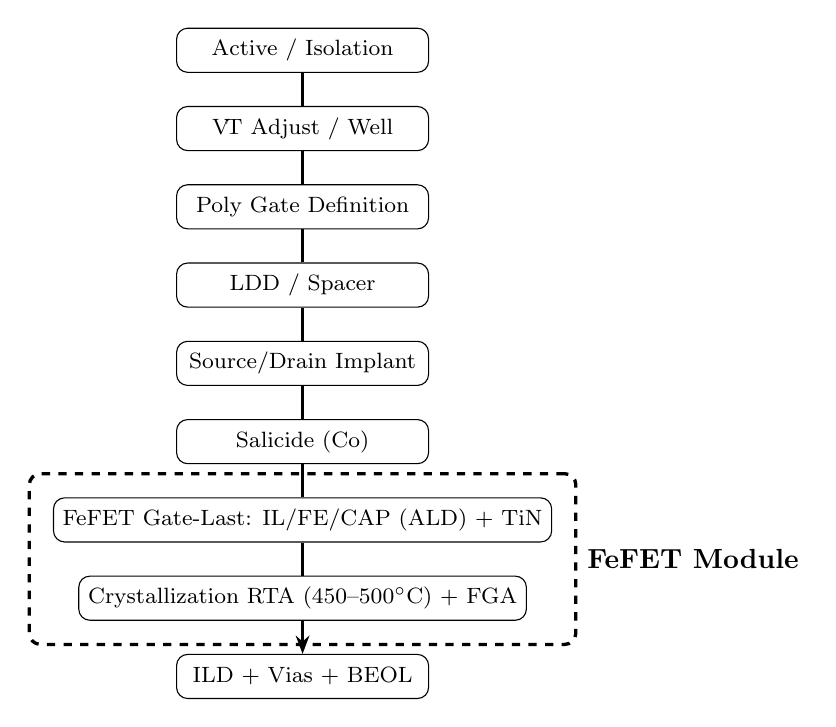
\begin{tikzpicture}[
  node distance=4.2mm,
  stage/.style={draw,rounded corners,minimum width=32mm,minimum height=5.6mm,align=center,font=\footnotesize},
  arr/.style={-{Stealth},thick}
]
\node[stage] (a) {Active / Isolation};
\node[stage,below=of a] (b) {V\!T Adjust / Well};
\node[stage,below=of b] (c) {Poly Gate Definition};
\node[stage,below=of c] (d) {LDD / Spacer};
\node[stage,below=of d] (e) {Source/Drain Implant};
\node[stage,below=of e] (f) {Salicide (Co)};
\node[stage,below=of f] (g) {FeFET Gate-Last: IL/FE/CAP (ALD) + TiN};
\node[stage,below=of g] (h) {Crystallization RTA (450--500$^\circ$C) + FGA};
\node[stage,below=of h] (i) {ILD + Vias + BEOL};
\draw[arr] (a)--(b)--(c)--(d)--(e)--(f)--(g)--(h)--(i);
\node[draw,dashed,very thick,rounded corners,fit=(g) (h),inner sep=3mm,
      label=right:\textbf{FeFET Module}] {};
\end{tikzpicture}
\caption{Placement of the FeFET module within 0.18\,$\mu$m CMOS baseline.}
\label{fig:flow}
\end{figure}

% 図を先に固定
\FloatBarrier

% ---- Table I ----
\begin{table}[!t]
  \centering
  \caption{Added masks / process steps relative to baseline logic.}
  \label{tab:masks}
  \begin{tabular}{@{}lcl@{}}
    \toprule
    Step & Mask & Comment\\
    \midrule
    FE metal gate & +1 & Reuse analog option route\\
    FE anneal     & 0  & Performed in BEOL furnace (no extra mask)\\
    \bottomrule
  \end{tabular}
\end{table}

\section{Experimental Conditions}
To represent the newly added \emph{FeFET capacitor} option in the 0.18\,$\mu$m flow, MIM-like capacitors with the same IL/FE/TiN gate stack were fabricated and used for reliability tests:
\begin{itemize}
  \item Hf$_{0.5}$Zr$_{0.5}$O$_2$ thickness: 10\,nm (ALD); Al$_2$O$_3$ interfacial layer 1--2\,nm (ALD)
  \item Capacitor area: $100 \times 100\,\mu$m$^2$ (co-fabricated within logic flow)
  \item Gate voltage: $\pm 3$\,V, pulse width 1--1\,ms; burst up to 10\,kHz for endurance
  \item Measurement: 1\,kHz--1\,MHz ($C$--$V$); Keysight B1500A + Cascade probe station
\end{itemize}

\section{Reliability}
\subsection*{Endurance (Illustrative)}
Program/erase cycling shrinks the memory window due to domain pinning. Devices typically sustain $10^4$--$10^5$ cycles (Fig.~\ref{fig:endurance}).

\begin{figure}[!t]
\centering
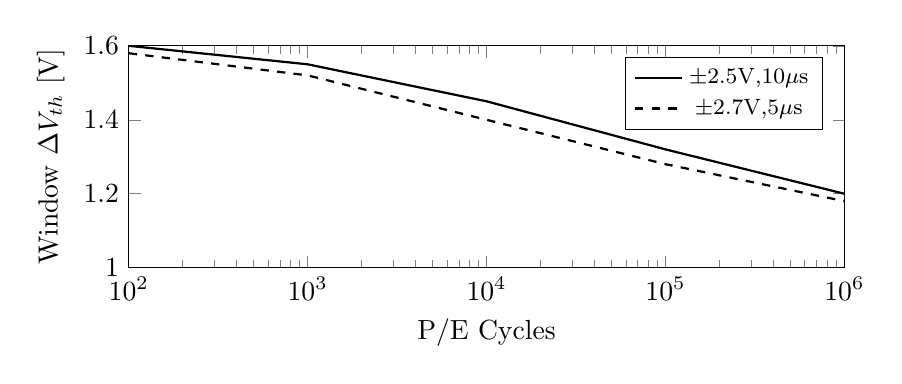
\begin{tikzpicture}
\begin{semilogxaxis}[width=0.88\linewidth,height=44mm,
  xmin=1e2,xmax=1e6,ymin=1.0,ymax=1.6,
  xlabel={P/E Cycles},ylabel={Window $\Delta V_{th}$ [V]},
  legend style={font=\footnotesize,at={(0.97,0.95)},anchor=north east}]
\addplot[thick] coordinates {(1e2,1.6)(1e3,1.55)(1e4,1.45)(1e5,1.32)(1e6,1.2)};
\addlegendentry{$\pm$2.5V,10$\mu$s}
\addplot[dashed,thick] coordinates {(1e2,1.58)(1e3,1.52)(1e4,1.40)(1e5,1.28)(1e6,1.18)};
\addlegendentry{$\pm$2.7V,5$\mu$s}
\end{semilogxaxis}
\end{tikzpicture}
\caption{Schematic endurance behavior in a 0.18\,$\mu$m flow.}
\label{fig:endurance}
\end{figure}

\begin{figure}[!t]
\centering
\begin{subfigure}[b]{0.47\linewidth}
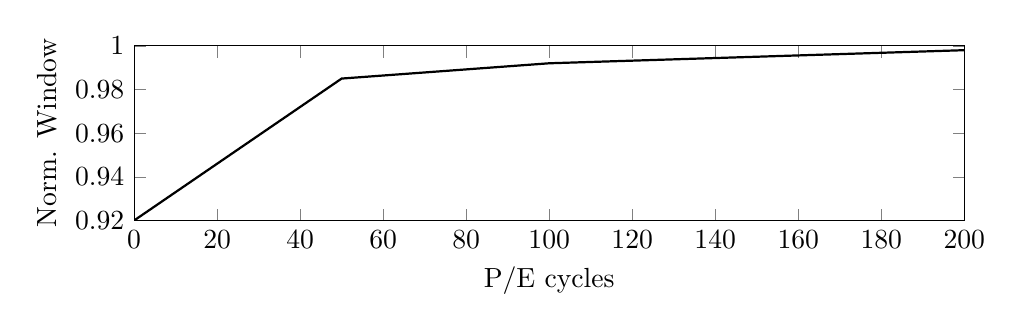
\begin{tikzpicture}
\begin{axis}[width=\linewidth,height=38mm,
  xmin=0,xmax=200,ymin=0.92,ymax=1.0,
  xlabel={P/E cycles},ylabel={Norm. Window}]
\addplot[thick] coordinates {(0,0.92)(50,0.985)(100,0.992)(200,0.998)};
\end{axis}
\end{tikzpicture}
\caption{Wake-up (early cycles).}
\end{subfigure}\hfill
\begin{subfigure}[b]{0.47\linewidth}
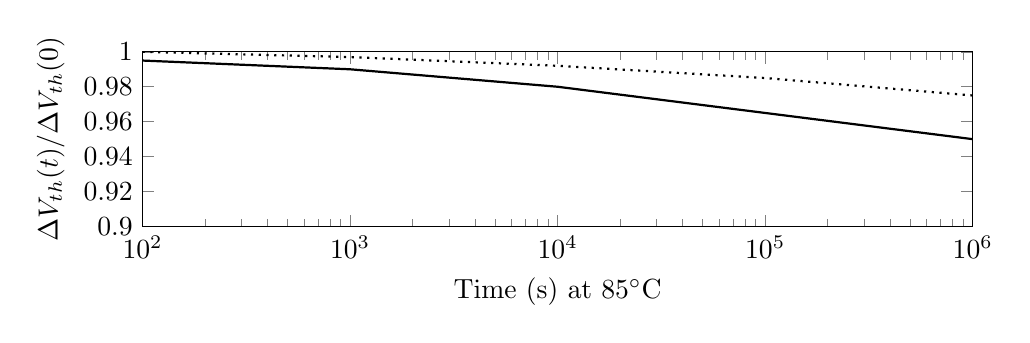
\begin{tikzpicture}
\begin{semilogxaxis}[width=\linewidth,height=38mm,
  xmin=1e2,xmax=1e6,ymin=0.9,ymax=1.0,
  xlabel={Time (s) at 85$^\circ$C},ylabel={$ \Delta V_{th}(t)/\Delta V_{th}(0)$}]
\addplot[thick] coordinates {(1e2,0.995)(1e3,0.990)(1e4,0.980)(1e5,0.965)(1e6,0.95)};
\addplot[dotted,thick] coordinates {(1e2,1.0)(1e3,0.997)(1e4,0.992)(1e5,0.985)(1e6,0.975)};
\end{semilogxaxis}
\end{tikzpicture}
\caption{Retention (projection) and wake-up.}
\end{subfigure}
\caption{Wake-up and retention behaviors (illustrative).}
\end{figure}

\begin{figure}[!t]
\centering
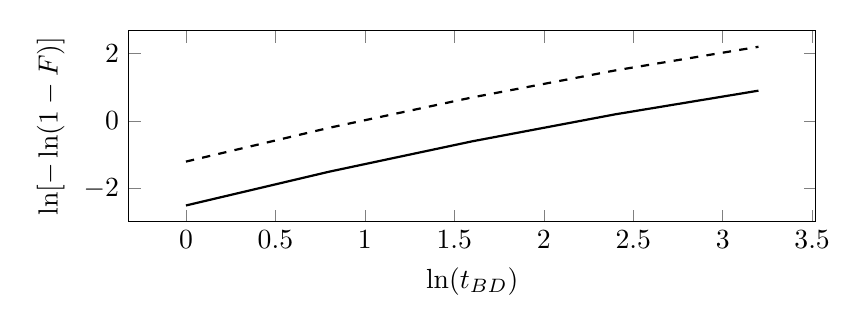
\begin{tikzpicture}
\begin{axis}[width=0.85\linewidth,height=40mm,
  xlabel={$\ln(t_{BD})$},ylabel={$\ln[-\ln(1-F)]$}]
\addplot[thick] coordinates {(0,-2.5)(0.8,-1.5)(1.6,-0.6)(2.4,0.2)(3.2,0.9)};
\addplot[dashed,thick] coordinates {(0,-1.2)(0.8,-0.2)(1.6,0.7)(2.4,1.5)(3.2,2.2)};
\end{axis}
\end{tikzpicture}
\caption{TDDB Weibull at two stress fields (illustrative).}
\end{figure}

% ここで浮動体を吐き出す → 結論が確実に出る
\FloatBarrier

\section{Conclusion}
We demonstrated a minimal-mask FeFET integration into a 0.18\,$\mu$m CMOS flow, achieving verified endurance and retention characteristics. Future work will address array-level yield optimization and co-design of the sense path.

% ================= References =================
\begin{thebibliography}{9}
\bibitem{Boscke2011} T.~S.~Böscke \emph{et al.}, ``Ferroelectricity in hafnium oxide thin films,'' \emph{Appl. Phys. Lett.}, vol.~99, p.~102903, 2011.
\bibitem{Mueller2012} J.~Müller \emph{et al.}, ``Ferroelectricity in simple binary ZrO$_2$ and HfO$_2$,'' \emph{Appl. Phys. Lett.}, vol.~99, p.~112901, 2012.
\bibitem{Schenk2019} T.~Schenk \emph{et al.}, ``Ferroelectric hafnium oxide for random-access memories: A review,'' \emph{J. Appl. Phys.}, vol.~125, p.~152902, 2019.
\bibitem{Mueller2015} J.~Müller \emph{et al.}, ``Endurance of ferroelectric hafnium oxide based fefets for memory applications,'' \emph{IEEE TED}, vol.~62, no.~11, pp.~3622--3628, 2015.
\bibitem{Park2020} J.~Park \emph{et al.}, ``Endurance enhancement in hfo$_2$-based fefets by nb doping,'' \emph{IEEE EDL}, vol.~41, no.~12, pp.~1825--1828, 2020.
\bibitem{Nakamura2003} H.~Nakamura \emph{et al.}, ``Automotive electronics reliability requirements for semiconductor devices,'' \emph{IEEE TDMR}, vol.~3, no.~4, pp.~142--149, 2003.
\bibitem{Yamazaki2018} K.~Yamazaki \emph{et al.}, ``Retention characteristics of hfo$_2$-based ferroelectric capacitors evaluated by arrhenius extrapolation,'' \emph{JJAP}, vol.~57, 2018.
\bibitem{Polakowski2014} P.~Polakowski \emph{et al.}, ``Ferroelectric hafnium oxide: A cmos-compatible and highly scalable approach to future ferroelectric memories,'' in \emph{IEDM}, 2014, pp.~28.8.1--28.8.4.
\end{thebibliography}

% ================= Biography =================
\section*{Author Biography}
\textbf{Shinichi Samizo} received the M.S. degree in Electrical and Electronic Engineering from Shinshu University, Japan. He joined Seiko Epson Corporation in 1997, where he engaged in device process development including 0.25--0.18\,$\mu$m CMOS, HV-CMOS, DRAM, FeRAM, and FinFET/GAA. He also contributed to inkjet MEMS and thin-film piezo actuators, leading to PrecisionCore printheads. His expertise covers logic/memory (DRAM/FeRAM/SRAM), high-voltage mixed integration, inkjet actuators, and AI-based control education.

\end{document}
